\documentclass[a4paper, 14pt]{article}

% !TEX root = main.tex

\DeclareUnicodeCharacter{03BB}{\ensuremath{\lambda}}
\DeclareUnicodeCharacter{03B7}{\ensuremath{\eta}}
\DeclareUnicodeCharacter{03C4}{\ensuremath{\tau}}
\DeclareUnicodeCharacter{03C1}{\ensuremath{\rho}}
\DeclareUnicodeCharacter{03F0}{\ensuremath{\kappa}}
\DeclareUnicodeCharacter{03BC}{\ensuremath{\mu}}

%%% Работа с русским языком
\usepackage{cmap}					% поиск в PDF
\usepackage{mathtext} 				% русские буквы в формулах
\usepackage[T2A]{fontenc}			% кодировка
\usepackage[utf8]{inputenc}			% кодировка исходного текста
\usepackage[english, russian]{babel}	% локализация и переносы
\usepackage[14pt]{extsizes}
\renewcommand{\rmdefault}{ptm}

\usepackage{caption}
\DeclareCaptionFont{white}{\color{white}}
\DeclareCaptionFormat{listing}{\colorbox{gray}{\parbox{\textwidth}{#1#2#3}}}
\captionsetup[lstlisting]{format=listing,labelfont=white,textfont=white}

\usepackage{hyperref}
\usepackage{titlesec}
\usepackage{amsmath, amsfonts, amssymb, mathtools} 

%%% Поля страницы
\usepackage[top=20mm, bottom=20mm, left=30mm, right=10mm, headsep=0pt]{geometry}
%\RequirePackage[left=30mm,right=10mm,top=20mm,bottom=20mm,headsep=0pt,includefoot]{geometry}

%%% Полуторный интервал
\usepackage{setspace}
\onehalfspacing

%%% Абзацные отступы
\usepackage{indentfirst} 

\usepackage{multirow}

%%% Вставка иллюстраций
\usepackage{graphicx}
\graphicspath{{img/}}

\titleformat{\section}
{\bfseries\Large}{\thesection}{1em}{}

\titleformat{\subsection}
{\bfseries\Large}{\thesubsection}{1em}{}

\titleformat{\subsubsection}
{\bfseries\Large}{\thesubsubsection}{1em}{}

%%% Код
\usepackage{listings,listingsutf8}
\newcommand{\specialcell}[2][c]{%
\begin{tabular}[#1]{@{}c@{}}#2\end{tabular}}
\newcommand{\anonsection}[1]{\section*{#1}\addcontentsline{toc}{section}{#1}}
\lstset{
	rulesepcolor=\color{black},
	rulecolor=\color{black},
	keywordstyle=\color{black}\bfseries,
	basicstyle=\color{black}\ttfamily\small,
	stringstyle=\color{black}\bfseries,
	frame = single,
	showstringspaces=false,
	breaklines=true,
	xleftmargin=15pt, 
	framexleftmargin = 0pt,
	framextopmargin = 10pt,
	framexbottommargin = 10pt,
	literate={а}{{\selectfont\char224}}1
	{б}{{\selectfont\char225}}1
	{в}{{\selectfont\char226}}1
	{г}{{\selectfont\char227}}1
	{д}{{\selectfont\char228}}1
	{е}{{\selectfont\char229}}1
	{ё}{{\"e}}1
	{ж}{{\selectfont\char230}}1
	{з}{{\selectfont\char231}}1
	{и}{{\selectfont\char232}}1
	{й}{{\selectfont\char233}}1
	{к}{{\selectfont\char234}}1
	{л}{{\selectfont\char235}}1
	{м}{{\selectfont\char236}}1
	{н}{{\selectfont\char237}}1
	{о}{{\selectfont\char238}}1
	{п}{{\selectfont\char239}}1
	{р}{{\selectfont\char240}}1
	{с}{{\selectfont\char241}}1
	{т}{{\selectfont\char242}}1
	{у}{{\selectfont\char243}}1
	{ф}{{\selectfont\char244}}1
	{х}{{\selectfont\char245}}1
	{ц}{{\selectfont\char246}}1
	{ч}{{\selectfont\char247}}1
	{ш}{{\selectfont\char248}}1
	{щ}{{\selectfont\char249}}1
	{ъ}{{\selectfont\char250}}1
	{ы}{{\selectfont\char251}}1
	{ь}{{\selectfont\char252}}1
	{э}{{\selectfont\char253}}1
	{ю}{{\selectfont\char254}}1
	{я}{{\selectfont\char255}}1
	{А}{{\selectfont\char192}}1
	{Б}{{\selectfont\char193}}1
	{В}{{\selectfont\char194}}1
	{Г}{{\selectfont\char195}}1
	{Д}{{\selectfont\char196}}1
	{Е}{{\selectfont\char197}}1
	{Ё}{{\"E}}1
	{Ж}{{\selectfont\char198}}1
	{З}{{\selectfont\char199}}1
	{И}{{\selectfont\char200}}1
	{Й}{{\selectfont\char201}}1
	{К}{{\selectfont\char202}}1
	{Л}{{\selectfont\char203}}1
	{М}{{\selectfont\char204}}1
	{Н}{{\selectfont\char205}}1
	{О}{{\selectfont\char206}}1
	{П}{{\selectfont\char207}}1
	{Р}{{\selectfont\char208}}1
	{С}{{\selectfont\char209}}1
	{Т}{{\selectfont\char210}}1
	{У}{{\selectfont\char211}}1
	{Ф}{{\selectfont\char212}}1
	{Х}{{\selectfont\char213}}1
	{Ц}{{\selectfont\char214}}1
	{Ч}{{\selectfont\char215}}1
	{Ш}{{\selectfont\char216}}1
	{Щ}{{\selectfont\char217}}1
	{Ъ}{{\selectfont\char218}}1
	{Ы}{{\selectfont\char219}}1
	{Ь}{{\selectfont\char220}}1
	{Э}{{\selectfont\char221}}1
	{Ю}{{\selectfont\char222}}1
	{Я}{{\selectfont\char223}}1
}

\newcommand{\biglisting}[1]{%
    \lstinputlisting[numbers=left]{#1}%
}

\sloppy

\usepackage[T2A, T1]{fontenc}
\usepackage[utf8]{inputenc}
\usepackage[english,russian]{babel}
\usepackage{misccorr}
\usepackage{graphicx}
\usepackage{amsmath}
\usepackage{amsfonts}
\usepackage{verbatim}
\usepackage{listings}
\usepackage{pgfplots}
\usepackage{graphicx}
\usepackage{pdfpages}

\usepackage{algorithm}
\usepackage{algpseudocode}


\begin{document}
    \begin{center}
	Министерство науки и высшего образования Российской Федерации
	
	
	Федеральное государственное бюджетное образовательное учреждение высшего образования
	
	
	«Московский государственный технический университет имени Н.Э.Баумана
	
	
	(национальный исследовательский университет)» (МГТУ им. Н.Э.Баумана)
\end{center}

\vspace{8ex}

\begin{flushleft}
	Факультет: "Информатика и системы управления"
	
	Кафедра: "Программное обеспечение ЭВМ и информационные технологии"
	
	Дисциплина: "Экономика программной инженерии"
\end{flushleft}
\vspace{5ex}
\begin{center}
	Отчет
	
	"Планирование программного проекта в Microsoft Project: настройка рабочей среды и создание нового проекта"
\end{center}

\vspace{5ex}

\begin{flushright}
	Студент: Барсуков Н.М.
	
	Группа: ИУ7-86Б
	
	Преподаватели: Барышникова М.Ю. 
	
	Силантьева А.В.
\end{flushright}
    \newpage
    \tableofcontents
    \section{Теоретическая часть}

\begin{figure}[h]
	\centering
	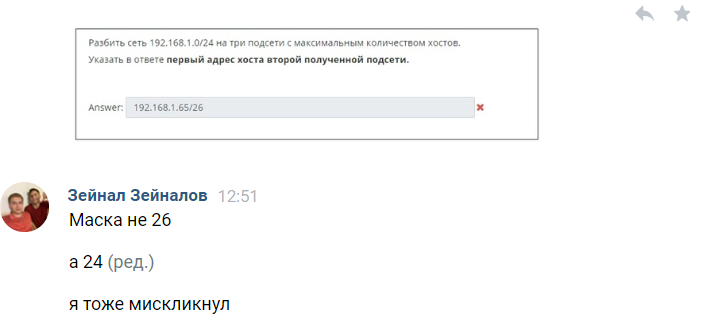
\includegraphics[width=0.7\linewidth]{src/Снимок}
	\caption{}
	\label{fig:}
\end{figure}

\begin{figure}[h]
	\centering
	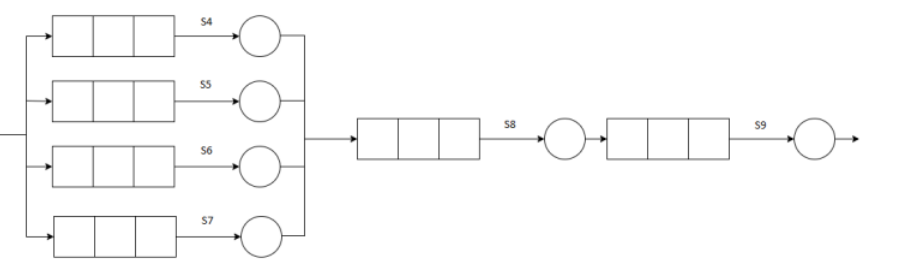
\includegraphics[width=0.7\linewidth]{src/Снимок1}
	\caption{}
	\label{fig:1}
\end{figure}

\begin{enumerate}
	\item S1, S2 – операторы;
	\item S3 – приём техники на починку;
	\item S4, S5, S6, S7 – восстановительные работы;
	\item S8 – отправка техники;
	\item S9 – выдача.
\end{enumerate}







\end{document}

\section{Заключение}

В ходе данного реферата были расмотрены приложения использующие технологию сетей. Рассмотрены различиные типологии организации сетей, сетевые модели и виды сетей.

